%%
%% This is file `mcmthesis-demo.tex',
%% generated with the docstrip utility.
%%
%% The original source files were:
%%
%% mcmthesis.dtx  (with options: `demo')
%%
%% -----------------------------------
%%
%% This is a generated file.
%%
%% Copyright (C)
%%     2010 -- 2015 by Zhaoli Wang
%%     2014 -- 2016 by Liam Huang
%%     2016 -- 2018 by Xuehan Sun
%%
%% This work may be distributed and/or modified under the
%% conditions of the LaTeX Project Public License, either version 1.3
%% of this license or (at your option) any later version.
%%
%% This work has the LPPL maintenance status `maintained'.
%%
%% The Current Maintainer of this work is Xuehan Sun.
%%
\documentclass{mcmthesis}
\mcmsetup{CTeX = false,   % 使用 CTeX 套装时,设置为 true
        tcn = 011, problem = B,
        sheet = true, titleinsheet = true, keywordsinsheet = true,
        titlepage = true}
\usepackage{palatino}
\usepackage{mwe}
\usepackage{graphicx}
\usepackage{subfig}
\usepackage{subcaption}
\usepackage{float}
\usepackage{multirow}
\usepackage{indentfirst}
\usepackage{gensymb}
\usepackage[ruled,lined,commentsnumbered]{algorithm2e}
\usepackage{geometry}
\geometry{left=2cm,right=2cm,top=2cm,bottom=2cm} %%页边距

\begin{document}
\linespread{0.6} %%行间距
\setlength{\parskip}{0.5\baselineskip} %%段间距
\title{Bus Booking Platform: A guarantee for quick leaving}

\date{\today}
	\begin{abstract}
	
     Located about 30 kilometres east of the city center, Pudong Airport
     occupies a 40-square-kilometre  site adjacent to the coastline
     in eastern Pudong. After years of growth on its passenger throughput and expansion of its site, Pudong Airport seems to let down its red-eye flight passengers, because of its weak evacuation capacity.
     
     To address this situation, our paper 
     
     We 
     
     Route Planning Model consists of two main submodels, namely Destination Selection Model, and Route Selection Model. For explanation, there are three figures showing steps and outcomes of it.
     
     Destination Selection Model aims to select potential destinations with MHA, based on population and transportation density. The final fifty destination stations are selected through KNN, and reasonable human revision.
     
     Route Selection Model use the outcomes of the former model, and employ Simulated Annealing to finalize our choice of routes.
     
     Bus Dispatching Model is aimed at arranging buses t
     
	 We use the Cost function to achieve a better result of user satisfaction and profits.
	
	 Afterwards, we make sensitivity analysis and discuss our model's strengths and weaknesses.
	 
	 In the end, we come up with an advertisement to promote our app: BusHub.
	
		\begin{keywords}
		destinations; route cycle selection; cost; order; BusHub
		\end{keywords}
	\end{abstract}

\maketitle

\tableofcontents

\newpage

\section{Introduction}
\subsection{Restatement of the Problem}
Shanghai Pudong International Airport is one of two international airports of Shanghai and a major aviation hub of China. Pudong Airport mainly serves international flights.

\begin{figure}[h]
    \centering
    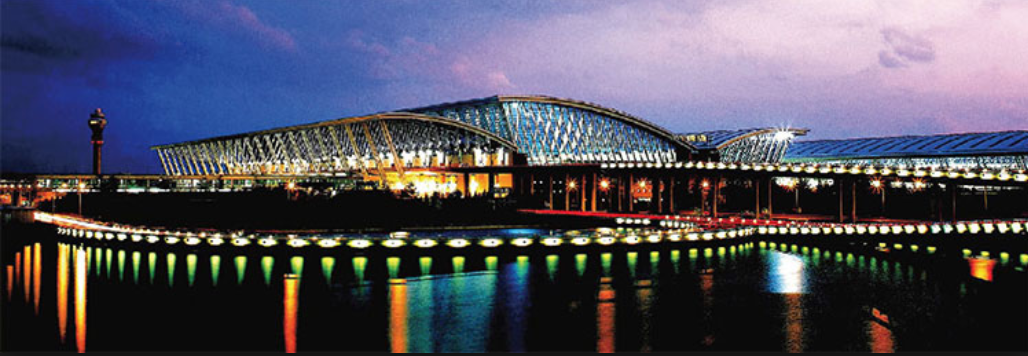
\includegraphics[width=0.8\textwidth]{SPIA.png}
    \caption{Shanghai Pudong International Airport \cite{Google_SPIA}}
    \label{fig:SPIA}
\end{figure}

As a huge rendezvous for many passengers, Pudong Airport has put forward a large number of measures to evacuate passengers. This operates quite well during daytime. However, during midnight period(23:00-02:00) when travellers get off from the red-eye flight, there is not enough transport capabilities to ensure passengers arrive home in a short time. According to official statistics from Shanghai Traffic Management Bureau(STMB), around 10,000 passengers are stranded at the airport, waiting for a home-ride for a long duration.

Therefore, a new service APP \emph{BusHub} is introduced by STMB to promote a higher-quality service. \emph{The bus-booking platform} dispatch orders and carefully pre-planned routes to each bus, relying on real-time demands from passengers. This leads to a shorter and cheaper commuting time, combining existing benefits of bus service and car-hailing.

\subsection{Our Work}
To better build the platform, we 



\section{Assumptions}

Our model makes four assumptions as follows:

\begin{enumerate}
	\item In the phase of modeling, we consider each passenger as the same individual subject, and the taxi and bus GPS data on January 31st, 2007 statistically representative. We assume each passenger has the same standard for user satisfaction, namely satisfied if bus is available while unsatisfied if not. Besides, we suppose there's little difference between the GPS data on the date we choose and others'.
	\item The GPS data typically reflects passengers' demands for buses' destinations. Since it's at deep night, there's few traffic jams. Besides, waiting time at the crossroads are randomly equal. 
	\item There is only one starting station, namely the Airport Station, and 50 terminal stations to choose from. All passengers need to go to this station to enjoy our bus-booking service. We don't take different airline landing site into account. 
	\item All the buses are the same, and seat 33 people. We simplify the bus to be used as the same standard bus, which has a fixed seat of thirty-three passengers averagely, based on our online research and calculation. Additionally, traffic accidents are ignored because it is rare, especially at night.
\end{enumerate}

\section{Nomenclature}
In this paper, we use the nomenclature in Table\ref{tab:Nomen} to describe our model. Other symbols that are used only once will be described later in the context.
\begin{table}
    \centering
    \caption{Nomenclature}
    \label{tab:Nomen}
    \begin{tabular}{c c}
\hline
    	Symbol & Definition\\
\hline
	$x$ & The longitude of each map point\\
	$y$ & The latitude of each map point\\
	$P(x,y)$ & The population density of each map point\\
	$T(x,y)$ & The taxi and bus GPS-recognized position density $i$\\
	$M(x,y)$ & The combined probability distribution of each map point\\
	$P_f$ & Acceptable risk ratio\\
	$Q(X_i;t)$ & Volumetric flow rate at time $t$ for dam $i$\\
\hline
    \end{tabular}
\end{table}





\section{Route Planning Model}

In this section, we will discuss our model of predefined route cycles. This model has two major aspects. To begin with, we investigate population density and transportation density of Shanghai to select potential destinations. Then, we provides potential routes for buses, based on selected destinations. This model achieves a great balance between cost and user satisfaction. Chongmin Island is not taken in account, because it's barely unseen in transpoatation density, and longitude, along wth latitude, is replaced by plane coordinates.

\subsection{Destination Selection Model}

In our model, we need to select 50 hot destinations for passengers to choose from as their destination station. $P(x,y)$ is generated through an officially given chart. We use the population density assigned to each color and color distribution, as well as noise reduction methods to get the two-dimension mathematical function. $T(x,y)$ is acquired through the given dataset. Form the given dataset, we assign a limited value to each existing map point. We take the longitude, latitude, speed, and status(occupied) into account, after which we apply convolution techniques to relevant values in order to form a two-dimension mathematical function. Both $P(x,y)$ and $T(x,y)$ is \textbf{normalized}

\begin{figure}[ht]
    \begin{minipage}{0.44\linewidth}
      \centerline{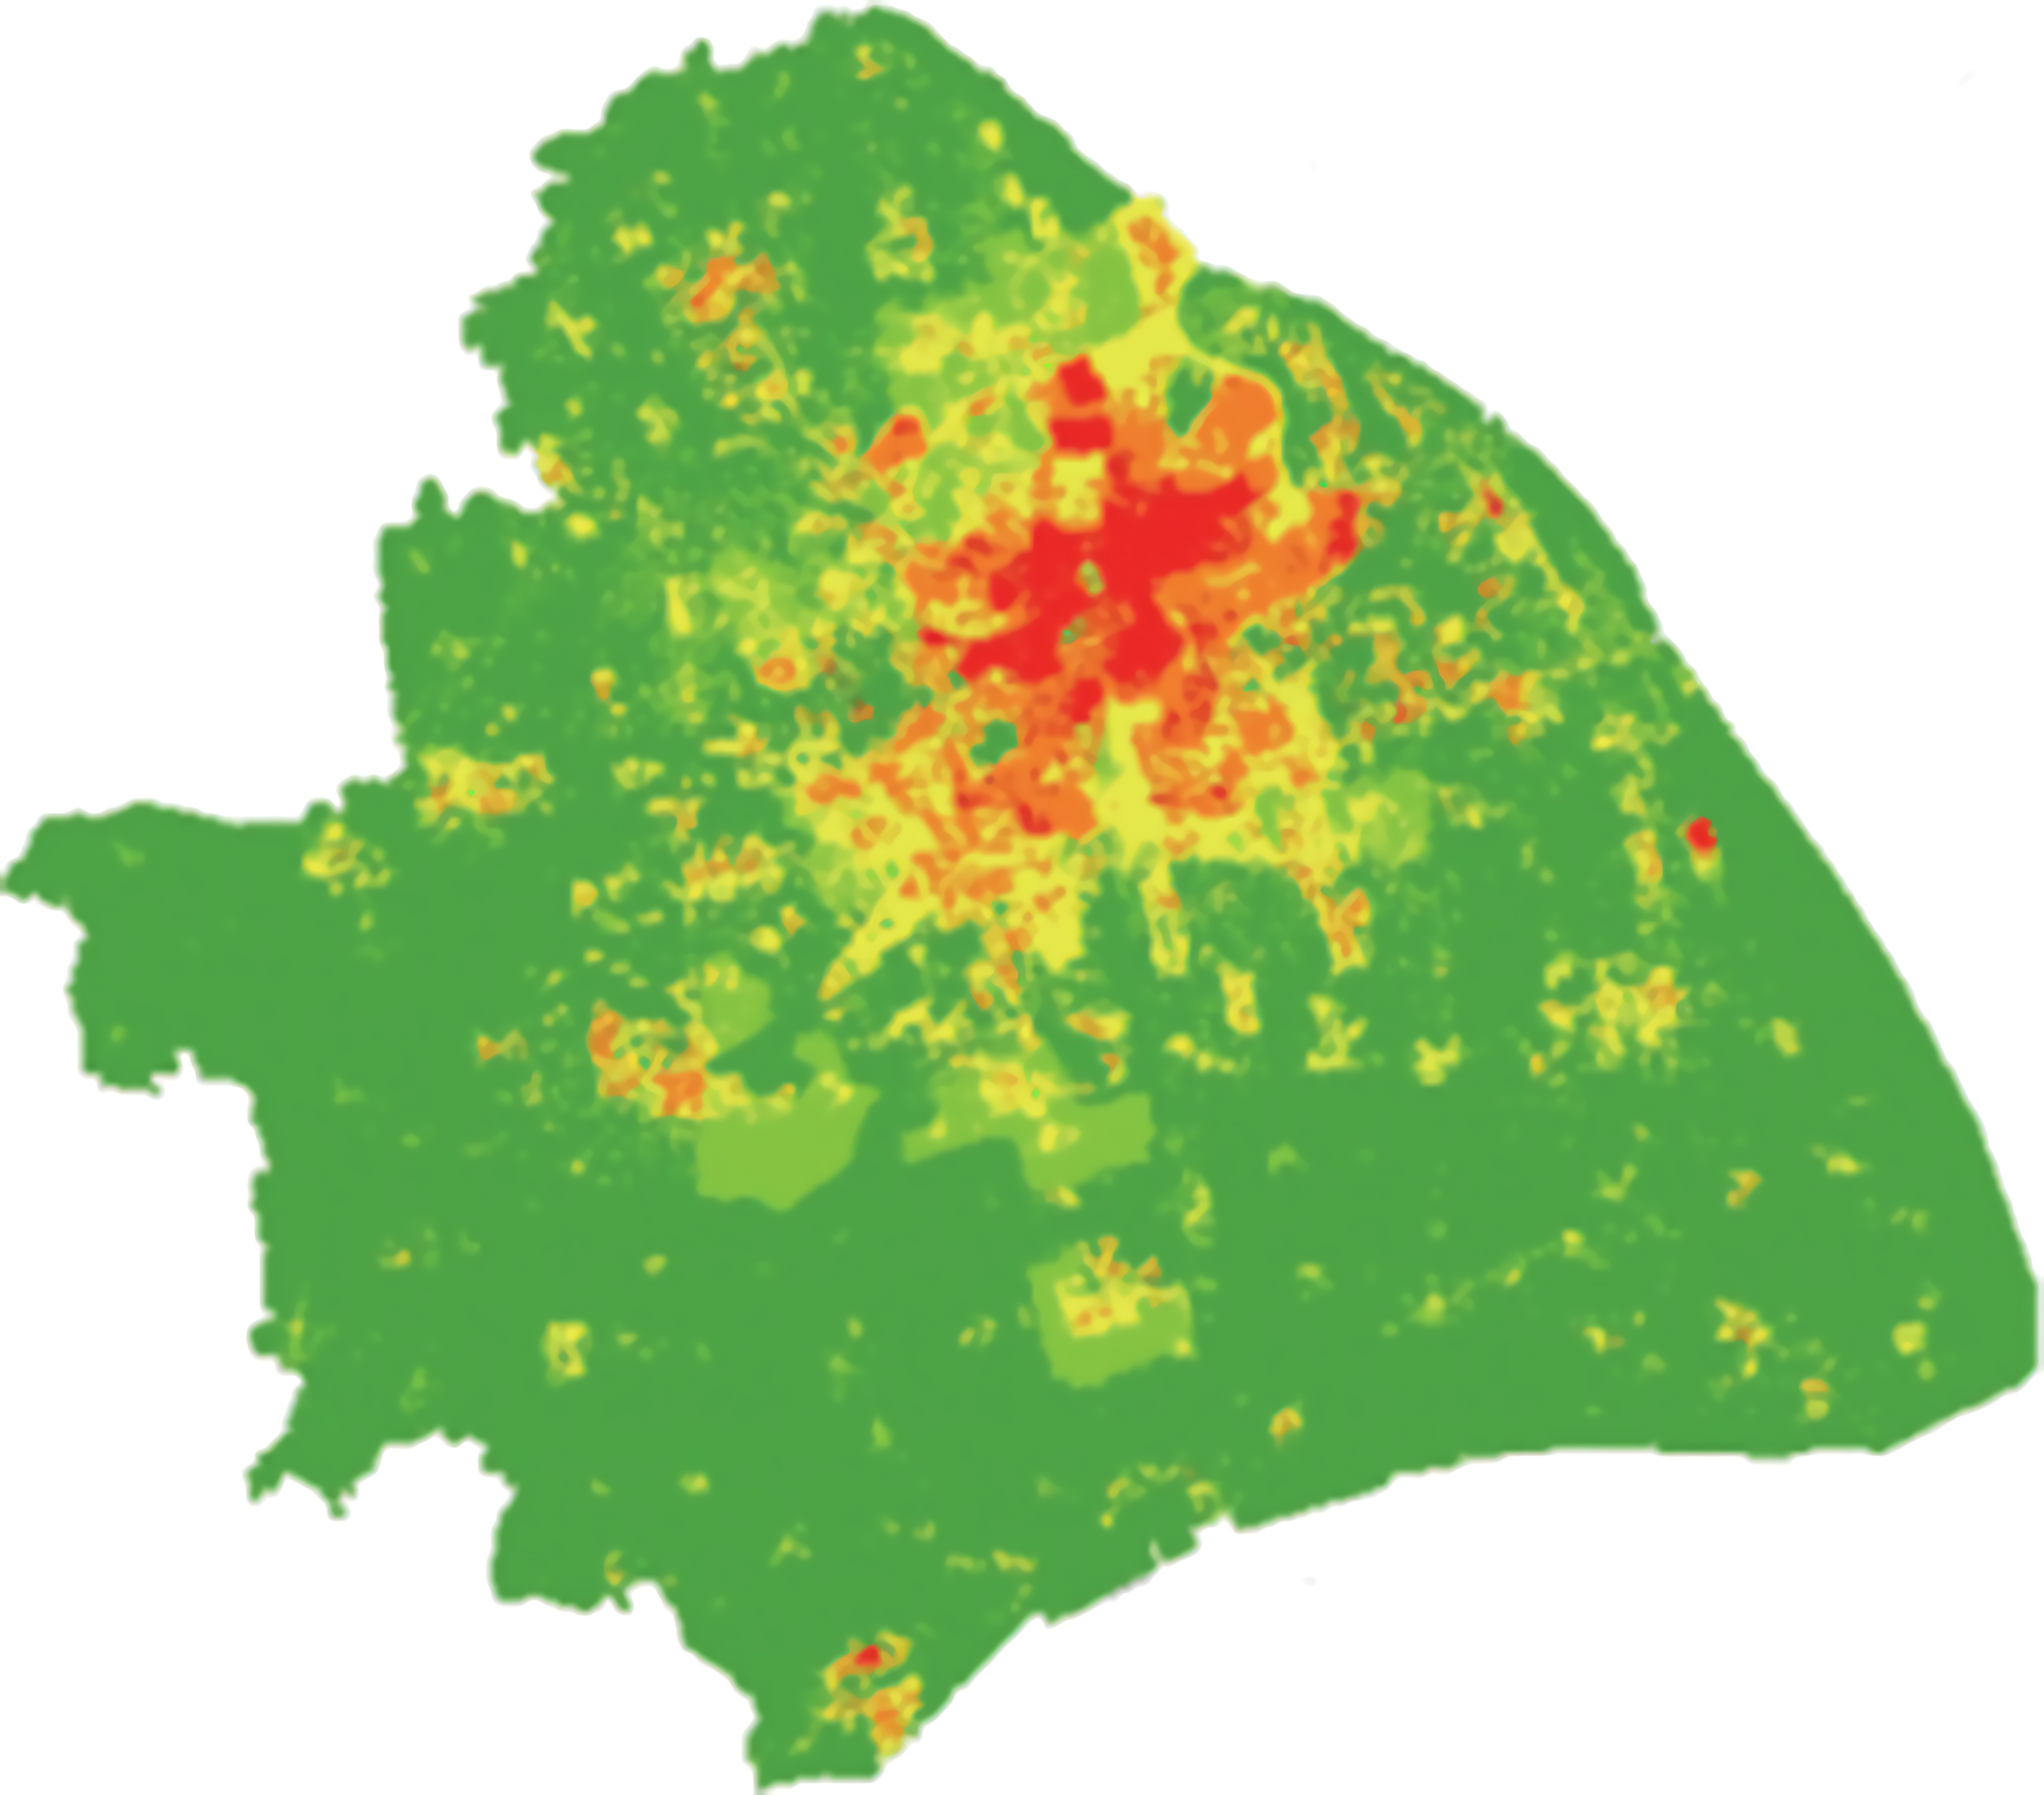
\includegraphics[height=5cm,width=6cm]{figures/Pd.jpg}}\cite{dqxxkx_ppl}
      \caption*{(a) Population Density of Shanghai.}
    \end{minipage}
    \hspace{0.5in}
    \begin{minipage}{0.44\linewidth}
      \centerline{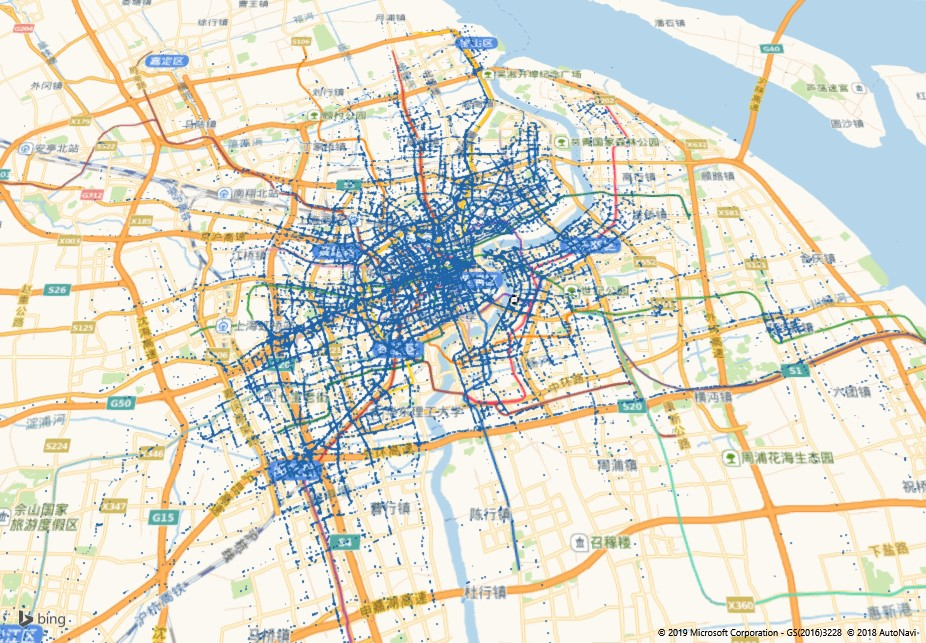
\includegraphics[height=5cm,width=6cm]{figures/Tran.png}}
      \caption*{(b) GPS-recognized Position Density.}
    \end{minipage}
    \caption{In figure(a), a red point means higher population density, while a green point means lower; In figure(b), each blue point represent a GPS-recognized position. This means the denser the blue points, the higher the position density.}
\end{figure}

We use the product of two functions as our final selection function to estimate potential destinations.

\begin{equation}\label{eq_product&sum}
    M(x,y) = \frac{P(x,y) \times T(x,y)}{P(x,y) + T(x,y)}
\end{equation}

For every map point $(x,y)$, the larger $M(x,y)$ is, the greater possibility for $(x,y)$ to be chosen as a destination. With this formula, we generate a chart on which we can preliminarily see the distribution of potential sites.

In order to get a smooth function of $P(x,y)$ and $T(x,y)$, Gaussian Low Pass Filter (GLPF)~\cite{DigitalImageProcessing} is applied to our sampling. The two-dimension version function of the filter is

\begin{equation}
    \begin{split}
      H(u,v)     & =   e^{-D^2(u,v)/2\sigma^2}\\
                 & =   e^{-9D^2(u,v)/2R^2}
    \end{split}
\end{equation}

where:
\begin{itemize}
\item $D(u,v)$ is the distance from the center of the frequency rectangle;
\item $\sigma$ is a measure of the degree of central expansion, which is equal to $\left( \frac{R}{3} \right)$;
\item $R$ is the precision radius, which is equal to 600 metres.
\end{itemize}

Then, we acquire a reasonable distribution of $M(x,y)$. Its picture is shown in Figure\ref{fig:M(x,y)}:

\begin{figure}[htbp]
    \centering
    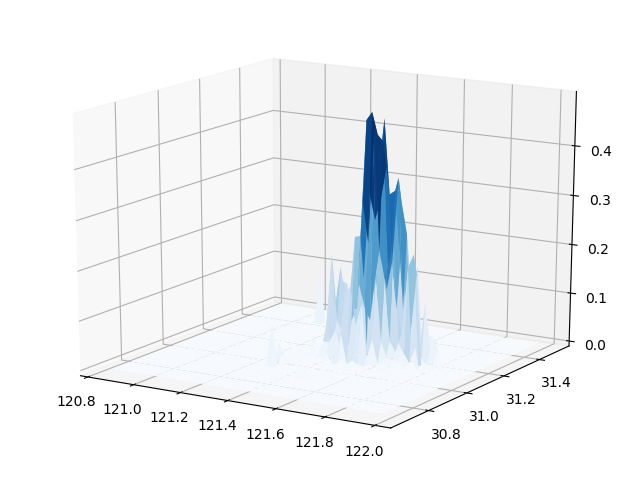
\includegraphics[height=5cm,width=7cm]{figures/M(x,y).png}
    \caption{Distribution of M(x,y)}
    \label{fig:M(x,y)}
\end{figure}

We employ \emph{Metropolis-Hasting Algorithm} to process the function M, and generate \textbf{potential destinations}. 

Afterward, \emph{K-Means Clustering} is applied to get fifty reasonable clusters, by which we finalize our selection of \textbf{50 destination stations}. Additionally, we also intervene the generation of these destinations

\begin{figure}[htbp]
    \begin{minipage}{0.44\linewidth}
      \centerline{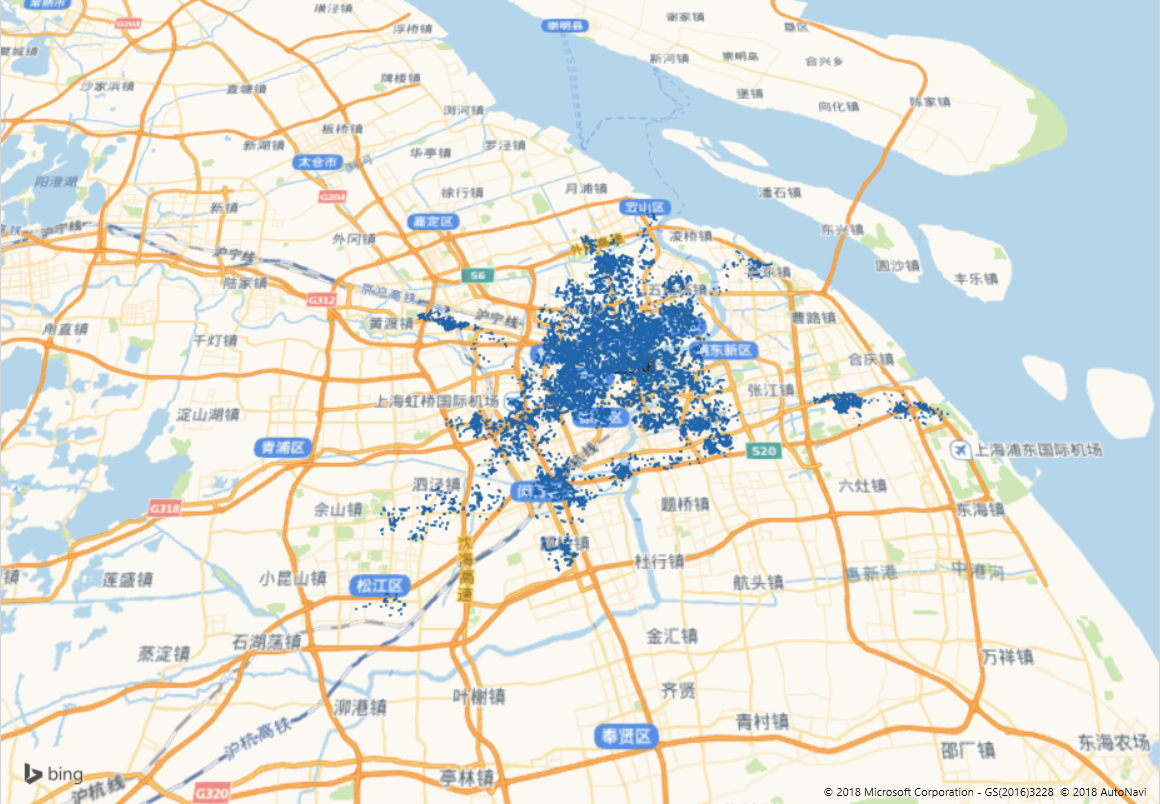
\includegraphics[height=5cm,width=7cm]{figures/PotentialDetinations.png}}
      \caption*{(a) Distribution of Potential Destinations.}
    \end{minipage}
    \hspace{0.5in}
    \begin{minipage}{0.44\linewidth}
      \centerline{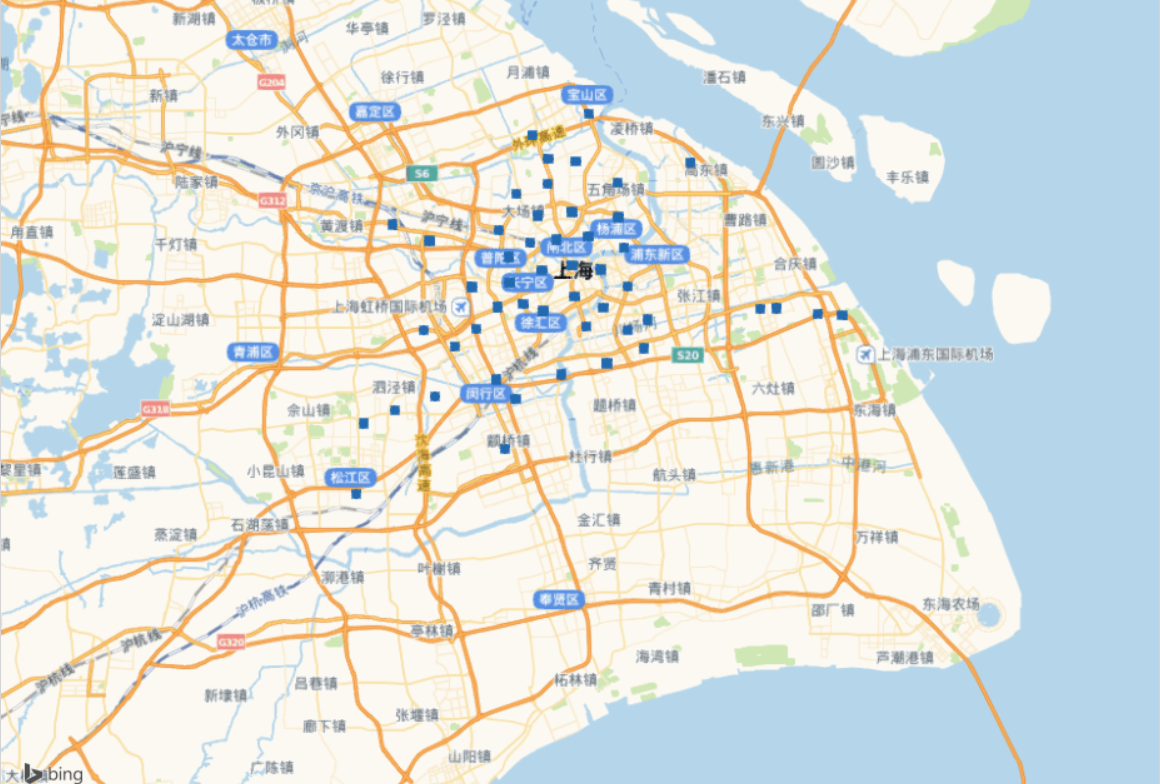
\includegraphics[height=5cm,width=7cm]{figures/fiftydestinations.png}}
      \caption*{(b) Distribution of fifty Destinations.}
    \end{minipage}
    \caption{Generation of fifty Destinations}
\end{figure}

\begin{figure}[htbp]
    \centering
    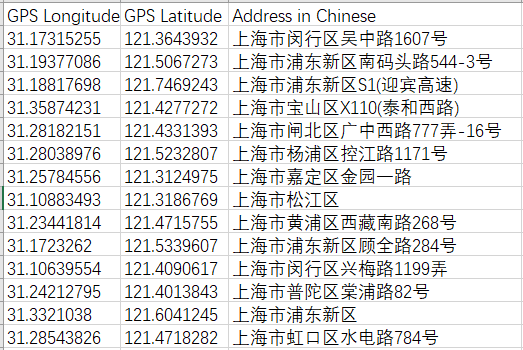
\includegraphics{figures/AddressinChinese.png}
    \caption{Part of the Destinations' Addresses in Chinese}
    \label{fig:AIC}
\end{figure}
We turn the destination address from the longitude-latitude form to detailed text address in Chinese. Thus, the APP can be more user-friendly. We extract a part of the total destinations shown in Figure\ref{fig:AIC}.

\subsection{Route Selection Model}
There are already potential destinations, and we consider each as a key knot. Possible route cycles only connect these knots.

\begin{equation}
\begin{aligned}	
    & \min\,\, Cost = \sum\limits_{Route\,\textbf{i}}(c_d \sum\limits_{e\in E_i} d_e + c_t \sum\limits_{e\in E_i} \frac{1}{t_e} + c_p \frac{1}{\sum\limits_{q\in Q_i} p_q})\\
    & s.t. \qquad
    \begin{cases}
    \bigcup\limits_{i}Q_i = Q & |Q| = 50,\\
    \bigcup\limits_{i}E_i = E & |E| = 50.
    \end{cases}
\end{aligned}
\end{equation}

where:
\begin{itemize}
    \item $e$, and $q$ are the corresponding elements of sets $E_i$ and $Q_i$;
    \item $E_i$ is the set of \textbf{edges} in \emph{route i};
    \item $Q_i$ is the set of points of destination stations we select;
    \item $d_e$ is the distance of each edge e.
\end{itemize}

We normalize $d_e$, $t_e$ and $p_q$ by applying:
\begin{equation*}
    \hat{D}=\frac{D - min}{max - min} \qquad \qquad \hat{X}=\frac{X}{\sum X_i}\left(\text{X=$d_e$ or $p_q$}\right)
\end{equation*}
The smaller $d_e$ is, the larger $t_e$ is, the bigger $p_q$ is, the less Cost function value is. This makes sense, since each bus has to be fueled per kilometre, and better traffic conditions as well as more seat occupan

\section{Bus Dispatching Model}



\section{Implementation}
\subsection{How our app works}





\section{Model Analysis}
\subsection{Sensitivity Analysis}

$\sigma$$AHP$

\subsection{Strengths and Weaknesses}
\subsubsection{Strengths}
\begin{enumerate}
    \item 
    \item

\end{enumerate}

\subsubsection{Weaknesses}
\begin{enumerate}
    \item 
    \item

\end{enumerate}

\section{Conclusion}
Our paper provides a detailed analysis of

\newpage
\section{Advertisement}
Bushub is a novel \emph{Bus Booking Platform} App. We aim to offer each passenger off the plane a quick arrival at the destination. \\
Advantages:
\begin{figure}[htbp]
    \centering
    
\includegraphics[height=6cm,width=10cm]{figures/Bushublogo.png}
\end{figure}

\subsection{Usage}
\begin{itemize}
\item Destinations: There are 50 destinations. You can see them through the qr code.
\item Price \& Time Intervals: Different destinations have different fares, which are in positive correlation to their distance. Time intervals are not fixed, since it relates to arrivals of flights, but we can offer you an approximate time, based on our model.
\item Download: Bushub is available on both App Store and Android Market.
\end{itemize}
\subsection{Best regards \& wishes}
We wish you a happy journey. For any further inquiries, please call:
\begin{figure}[hbtp]
    \centering
    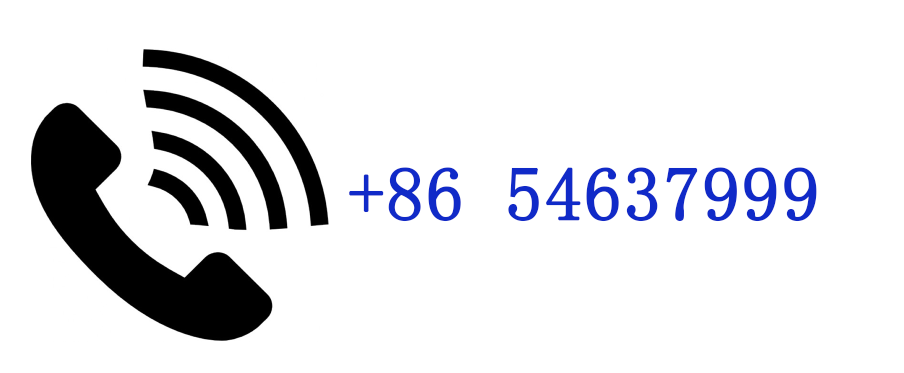
\includegraphics[height=2cm,width=7cm]{figures/Bushubtele.png}
\end{figure}



\newpage
	\bibliographystyle{IEEEtran}
	\bibliography{newrefs}
	
	
	
	
	
\newpage
\begin{appendices}
\section{Fifty Selected Destinations}
% Table generated by Excel2LaTeX from sheet 'Stations'
\begin{table}[htbp]
  \centering
  \caption{Longitude and Latitude of Fifty Destinations}
    \begin{tabular}{l|r}
    \multicolumn{2}{c}{Fifty Destination Stations} \\
    Longitude & Latitude \\
    121.364393162531  \qquad \qquad \qquad & \qquad \qquad \qquad 31.173152552460  \\
    121.506727261692  \qquad \qquad \qquad & \qquad \qquad \qquad 31.193770863610  \\
    121.746924348685  \qquad \qquad \qquad & \qquad \qquad \qquad 31.188176982499  \\
    121.427727151510  \qquad \qquad \qquad & \qquad \qquad \qquad 31.358742313098  \\
    121.433139324850  \qquad \qquad \qquad & \qquad \qquad \qquad 31.281821514808  \\
    121.523280704171  \qquad \qquad \qquad & \qquad \qquad \qquad 31.280389760460  \\
    121.312497485300  \qquad \qquad \qquad & \qquad \qquad \qquad 31.257845558004  \\
    121.318676931596  \qquad \qquad \qquad & \qquad \qquad \qquad 31.108834932138  \\
    121.471575456181  \qquad \qquad \qquad & \qquad \qquad \qquad 31.234418142819  \\
    121.533960720319  \qquad \qquad \qquad & \qquad \qquad \qquad 31.172326196662  \\
    121.409061703513  \qquad \qquad \qquad & \qquad \qquad \qquad 31.106395542063  \\
    121.401384292276  \qquad \qquad \qquad & \qquad \qquad \qquad 31.242127947224  \\
    121.604124514158  \qquad \qquad \qquad & \qquad \qquad \qquad 31.332103796933  \\
    121.471828168427  \qquad \qquad \qquad & \qquad \qquad \qquad 31.285438256653  \\
    121.230262324458  \qquad \qquad \qquad & \qquad \qquad \qquad 31.015230791544  \\
    121.700675726468  \qquad \qquad \qquad & \qquad \qquad \qquad 31.193410339600  \\
    121.238600547066  \qquad \qquad \qquad & \qquad \qquad \qquad 31.083179839898  \\
    121.489783526947  \qquad \qquad \qquad & \qquad \qquad \qquad 31.262117133953  \\
    121.402093037180  \qquad \qquad \qquad & \qquad \qquad \qquad 31.218021052389  \\
    121.438025579592  \qquad \qquad \qquad & \qquad \qquad \qquad 31.229559793646  \\
    121.459520619477  \qquad \qquad \qquad & \qquad \qquad \qquad 31.129833350839  \\
    121.271084910573  \qquad \qquad \qquad & \qquad \qquad \qquad 31.273177521576  \\
    121.445246934034  \qquad \qquad \qquad & \qquad \qquad \qquad 31.336013691238  \\
    121.529393896826  \qquad \qquad \qquad & \qquad \qquad \qquad 31.251364350760  \\
    121.387172859152  \qquad \qquad \qquad & \qquad \qquad \qquad 31.124929047336  \\
    121.439640469256  \qquad \qquad \qquad & \qquad \qquad \qquad 31.191039080854  \\
    121.306396260030  \qquad \qquad \qquad & \qquad \qquad \qquad 31.172488372549  \\
    121.476011627950  \qquad \qquad \qquad & \qquad \qquad \qquad 31.333448666715  \\
    121.397037102902  \qquad \qquad \qquad & \qquad \qquad \qquad 31.058798512089  \\
    121.522513215793  \qquad \qquad \qquad & \qquad \qquad \qquad 31.313030242158  \\
    121.454646336302  \qquad \qquad \qquad & \qquad \qquad \qquad 31.258801946350  \\
    121.487640064119  \qquad \qquad \qquad & \qquad \qquad \qquad 31.176185161081  \\
    121.388412091579  \qquad \qquad \qquad & \qquad \qquad \qquad 31.194354995338  \\
    121.390018516950  \qquad \qquad \qquad & \qquad \qquad \qquad 31.267699508414  \\
    121.341503761017  \qquad \qquad \qquad & \qquad \qquad \qquad 31.156572158483  \\
    121.556704519879  \qquad \qquad \qquad & \qquad \qquad \qquad 31.182669427071  \\
    121.773870135207  \qquad \qquad \qquad & \qquad \qquad \qquad 31.186969896870  \\
    121.552350935580  \qquad \qquad \qquad & \qquad \qquad \qquad 31.154895396208  \\
    121.273777676284  \qquad \qquad \qquad & \qquad \qquad \qquad 31.096099848443  \\
    121.425089224955  \qquad \qquad \qquad & \qquad \qquad \qquad 31.256263202675  \\
    121.409972105050  \qquad \qquad \qquad & \qquad \qquad \qquad 31.302694807414  \\
    121.359945503646  \qquad \qquad \qquad & \qquad \qquad \qquad 31.213554954933  \\
    121.504103558526  \qquad \qquad \qquad & \qquad \qquad \qquad 31.230112052397  \\
    121.444298701623  \qquad \qquad \qquad & \qquad \qquad \qquad 31.312259258587  \\
    121.417223173704  \qquad \qquad \qquad & \qquad \qquad \qquad 31.197270242250  \\
    121.511163311648  \qquad \qquad \qquad & \qquad \qquad \qquad 31.140525418237  \\
    121.533558672333  \qquad \qquad \qquad & \qquad \qquad \qquad 31.213915495691  \\
    121.681836497288  \qquad \qquad \qquad & \qquad \qquad \qquad 31.192687075444  \\
    121.474509588538  \qquad \qquad \qquad & \qquad \qquad \qquad 31.204650653065  \\
    121.491086492494  \qquad \qquad \qquad & \qquad \qquad \qquad 31.378981942682  \\
    \end{tabular}%
  \label{tab:addlabel}%
\end{table}%

\end{appendices}
\end{document}


